\documentclass[12pt]{article}
\usepackage{times}
\usepackage{amsmath}
\usepackage{amssymb}
% \usepackage[pdftex]{graphicx} % Need this for MAC, comment out for PC
% \usepackage{epstopdf}         % Need this for MAC, comment out for PC
\usepackage{epsfig}           % Need this for PC, comment out for MAC
\usepackage{ITC}
\usepackage[caption=false]{subfig}

\title{\Large \vspace{-0.5in}
\MakeUppercase{Shape Detection in an Image using Parallelized Traditional Image Analysis Techniques}}
% {\footnotesize \textsuperscript{*}Note: Sub-titles are not captured in Xplore and should not be used}
% \thanks{Identify applicable funding agency here. If none, delete this.}}
\author{ Alan Manuel Loreto Cornídez, Rubén Diego Fuentes Gutiérrez\\
    \normalsize College of Electrical and Computer Engineering\\
    \normalsize The University of Arizona\\ 
    \normalsize Tucson, AZ, 85721\\
    \normalsize \{aloretocornidez,rfuentesgtz, mwm\}@arizona.edu\\[6pt]
    Faculty Advisor: Dr. Michael W Marcellin
  }

\date{}

\begin{document}

\maketitle


\section{\MakeUppercase{Abstract}}

\noindent
Modern day computer vision applications are frequently implemented using machine learning approaches.
However, when training data is not adequate or data is not application specific, performance of implementations can suffer.
This makes manual processing of the images a necessary step to retrieve the necessary shape data.
Image processing implementations are computationally intensive but highly parallelizable in nature and thus it is often ideal to implement them on heterogeneous computer architectures.
In this study, the Circle Detection Hough Transform was implemented on an NVIDIA 1070ti which resulted in a speedup of approximately 6950x for parameter space population of a 700$\times$700 pixel image when compared to a serial version implemented on an i7 8700K processor running at 4.7GHz.
Image pre-processing was also implemented in a heterogeneous fashion rendering an approximate 840x speedup with further optimizations rendering 1.44x and 1.5x speedups respectively. 


\section{\MakeUppercase{Introduction}}

\noindent
Modern image analysis algorithms are computationally intensive, generally requiring powerful system compute units and algorithms optimized for the application at hand in order to be effectively implemented in a system. 
The Hough Transform (HT)\cite{BALLARD1981111} - an algorithm used to parameterize shapes present in an image –- is one such algorithm that is computationally intensive for a traditional serial-style execution computer processing unit (CPU).
The algorithm requires that a parameter space be populated in order to detect shapes that are present in an edge map of the input image.
Image processing algorithms lend themselves to parallelization very well, and thus, GPUs are traditionally used in conjunction with CPUs to speed up image processing algorithm execution.
While upfront costs, such as memory transfer time, must be paid when utilizing heterogeneous computing architectures, overall execution time speedup still may occur due to faster computation when utilizing GPU hardware.
This makes programming end-to-end algorithms a viable option for when execution speedup is required for a specific application.








\section{\MakeUppercase{Related Work}}
\label{sec:relatedWork}
The HT contains many pre-processing algorithms that must be run on an input image that has objects that must be detected.
In our case, we want to detect the circles that are present in an image.
The image processing algorithms that are present in the HT include grayscale conversion, multiple instances of convolution and histogram generation of parameterized shapes.

\subsection{\MakeUppercase{Convolution}}
\label{sec:convolution}
% Many different implementations have been created for convolution. Chellapilla et al.\cite{document-parsing} implemented an unrolled loop for convolution operations.
% In addition, the Fast Fourier Transform has been used to convert the convolution operation into a multiplication operation\cite{vasilache2015fast}.
Other implementations\cite{9229640}of the convolution operation optimized the reduction of memory transactions.
Ultimately, our group decided to utilize tiling to conduct the matrix multiplications required for the convolution operation.

\subsection{\MakeUppercase{Histogram Generation}}
\label{subsec:histogramGeneration}
While methods have been implemented to assist with histogram generation, they have restrictions that are not applicable to the HT. 
The method proposed by Gocho and Arii\cite{9324376} is applicable to generating large histograms where the histogram values are dependent on multiple image pixel values.
On the other hand, Vetter and Westermann implement many of the similar histogram optimizations discussed in class.
Such as a local accumulator to reduce atomic operations and private histograms contained in shared memory to reduce memory contention. 
However, this implementation is not suited to streaming because of the memory access pattern \cite{5872623}. 

\begin{figure}%[t]
  \centering
  \subfloat[Input image containing circles.]{
  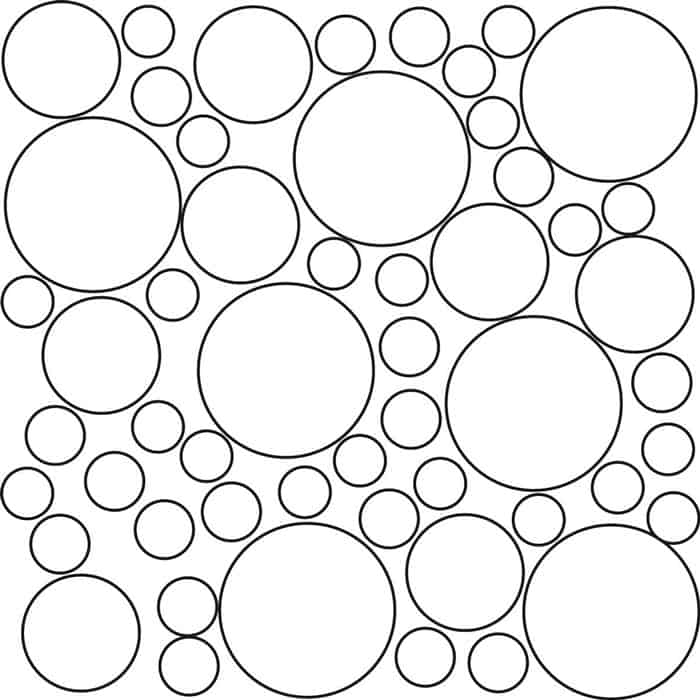
\includegraphics[width=2.5in]{figures/input-circles}\label{fig:input-circles}
  }
  \hfil
  \subfloat[Circles detected within the image.]{
  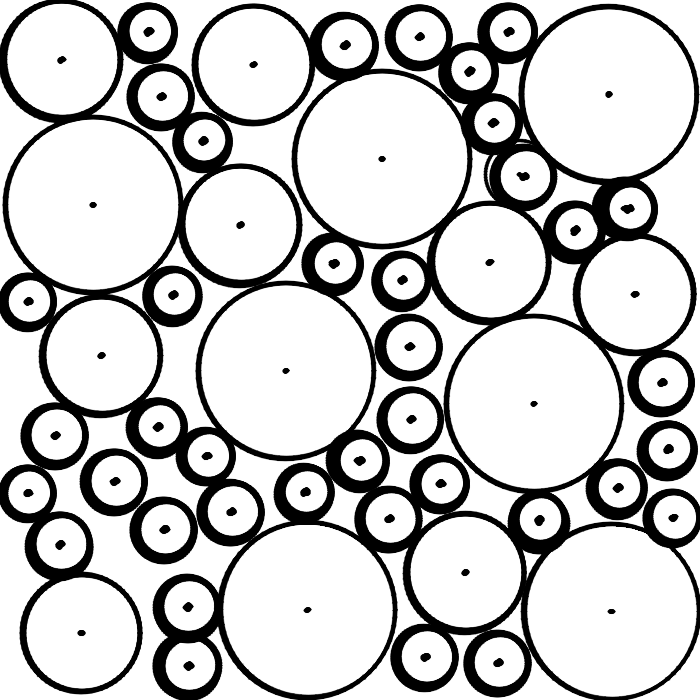
\includegraphics[width=2.5in]{figures/detected-circles}\label{fig:detected-circles}
  }
  \caption{\ref{fig:input-circles} is the input image that was used as an input to the program.\ref{fig:detected-circles} is the output to the program when it is run.}
\end{figure}


\section{\MakeUppercase{Methodology}}
\label{sec:Methodology}
% In this work, we 
% \subsection{The Hough Transform}
The HT implementation for our project detects circles that are present in an image compared to traditional line detection.
The HT itself is the population of a parameter space array, also referred to as an R-Table.
However, in order to run the population of the R-Table, multiple pre-processing routines are necessary to prepare the image for accurate shape detection.
% to occur on the input image before the parameter space, also referred to as the R-Table, can be populated.
The steps of the algorithm including pre-processing are color to grayscale conversion, edge detection, followed by population of the R-Table.
Our proposed method to implementing the HT includes using streaming in order to pipeline memory transfer with convolution calculations and R-Table population.





% Steps of the hough transform.
\begin{figure}
  \begin{itemize}
    \item RGB to Grayscale conversion of the input image.
    \item Image Blurring 
    \item Edge Map Generation
    \item Populate R-Table
  \end{itemize}\caption{Steps to conducting a Hough Transform on an image assuming an RGB image input.}\label{figure:hough-transform-steps}
\end{figure}

\subsection{RGB to Grayscale Conversion}
Grayscale conversion of an image lends itself well to parallelization depending on the encoding of the image.
In our case, the input image used an RGB-RGB pixel ordering scheme, allowing for coalesced memory accesses from the GPU's global memory.


\subsection{Convolution}
After generating the gray scale color space image, the majority of the algorithms used in image pre-processing for the HT can be applied via a convolution operation on the image.
Convolution is an algorithm that generates the convolution pixel by summing the element-wise multiplication of a source matrix and mask matrix as shown in \ref{equation:convolution}.

\begin{equation}
  m[x,y] * s[x,y] = \sum\limits_{i = 1}^{u} \sum\limits_{j = 1}^{v} m[i,j]s[x-i, y-j]
  \label{equation:convolution}
\end{equation}
Where $m$ is the mask matrix and $s$ is the source image matrix, $u$ and $v$ are the mask matrix dimensions. In our case, the mask matrices are square matrices.
Convolution is an algorithm that is readily parallelizable when implemented on a GPU, and as such, there were multiple optimizations that were made to extract as much performance as possible for image pre-processing.
Our convolution kernels were implemented in three iterations. 
A convolution kernel using global memory, one using constant memory for the mask, and a kernel utilizing shared memory stored in a 2D array.


\subsubsection*{Convolution Optimizations}
Convolution is a high-priority algorithm for the researchers' implementation.
Blurring, edge detection, and thresholding all feature convolution as the main algorithm component.
After careful analysis, it was determined that there was potential  for parallelization.
This is because convolution features many independent multiplications, and GPUs are purpose built for these kinds of applications.
In first iteration of the convolution kernel, the goal is to translate the serial code into a parallel framework.
To do this, a naive approach shall be taken as a baseline.
Each thread is mapped to a single pixel image, meaning that for a m x n image, m x n threads are used.
Each thread accesses surrounding pixels, as well as the convolution kernel (or mask).
Finally, once the computation is done, the result is stored back in global memory by the thread.
Bounds checking is primordial to properly operate on images with dimensions not evenly divisible by the block size.
As will be discussed in a later section, this provided significant performance benefits.
However, further optimizations are possible.
As was covered in the GPU memory hierarchy overview in a previous section, we seek to exploit the benefits of GPU architecture to the fullest.
A big component of convolution is the continuous access of the convolution kernel.
As such, the next proposition was to transfer constant convolution kernels to the constant memory.
Transferring the entire image was not a possibility, as the constant memory is very limited in capacity.
While constant memory did provide a performance improvement it was relatively minor, and much lower than anticipated (as discussed further below).
To further improve performance,  a shared memory implementation was needed.
There were some challenges to this, as thread blocks require more memory elements than there are threads in the block.
To counter this, more thread blocks were launched with each block working on less amount of data.
This improved performance to acceptable levels.


By using a variety of masks across the images, it is possible to extract features or generate new kinds of maps that can be utilized by the HT\@.
Image denoising and gradient maps are both results of convolution operations with different masks.

\subsubsection*{Image Blurring}
After the image is converted into grayscale color space, the image is de-noised by means of Gaussian blurring.
This aids in edge map generation by filtering our high frequency elements from the image.
To generate a blurred image, a convolution operation must be performed with a blurring mask. 
Our implementation uses a $5 \times 5$ Gaussian blurring mask where $\sigma = 1.4$ as shown in \ref{equation:gaussian5by5}.



\begin{figure} %[h] puts the figure 'here'
  \centering
  $\begin{bmatrix}
  0.01 & 0.22 & 0.03 & 0.22 & 0.01 \\
  0.22 & 0.04 & 0.06 & 0.04 & 0.22 \\
  0.03 & 0.06 & 0.08 & 0.06 & 0.03 \\
  0.22 & 0.04 & 0.06 & 0.04 & 0.22 \\
  0.01 & 0.22 & 0.03 & 0.22 & 0.01 \\
\end{bmatrix}$\caption{A $5 \times 5$ Gaussian blurring mask where $\sigma = 1.4$}\label{equation:gaussian5by5}
\end{figure}


\subsubsection{Gradient Map Generation}
After the image has been denoised by blurring, an edge map must be generated using two convolution operations using the horizontal\ref*{sub@equation:horizontalSobel} and  vertical\ref{sub@equation:verticalSobel} variations of the Sobel operator as shown in \ref{figure:sobelOperator}.
\begin{figure}[h] %[h] puts the figure 'here'
  \centering
  \subfloat[Horizontal Operator]{
  $\begin{bmatrix}
    -1 && -2 && -1 \\
    0 && 0 && 0 \\
    1 && 2 && 1 \\
  \end{bmatrix}$\label{equation:horizontalSobel}
  }
  \hfil
  \subfloat[Vertical Operator]{
  $\begin{bmatrix}
    -1 && 0 && 1 \\
    -2 && 0 && 2 \\
    -1 && 0 && 1 \\
  \end{bmatrix}$\label{equation:verticalSobel}
  }
  \caption{A $3 \times 3$ Sobel Operator}\label{figure:sobelOperator}
\end{figure}

\subsubsection{Grayscale Thesholding}
After the convolution operation is performed with both masks the horizontal gradient $G_x$ and vertical gradient $G_y$ are generated. 
The gradient magnitude can be calculated using the gradient magnitude, $G$, as shown in \ref{equation:gradientMagnitude}.

\begin{equation}
  G = \sqrt{{G_x}^2 + {G_y}^2}\label{equation:gradientMagnitude}
\end{equation}



% \section{\MakeUppercase{The Body}}
% \label{sec:NumericalResults}
% \section{\MakeUppercase{The Body}}
% \label{sec:NumericalResults}
% \section{\MakeUppercase{The Body}}
% \label{sec:NumericalResults}
% \section{\MakeUppercase{The Body}}
% \label{sec:NumericalResults}
% \section{\MakeUppercase{The Body}}
% \label{sec:NumericalResults}








\bibliographystyle{ieeetr}
\bibliography{references.bib}
\end{document}
